\chapter {Estudis i propostes de disseny}

\section {Disseny esquem�tic del sistema}
Disseny a tres capes:
	Frontend	VFS
	Adaptaci�	(definici� d'una interf�cie)
	Backend		Clustering (implementaci� de la interf�cie depenent del sistema de
clustering)

\subsection{Frontend}

Implementaci� de la jerarquia generica d'administraci� a trav�s de les funcions
que proporciona l'abstracci�
(sistema de fitxers virtual) del sistema sobre el que s'executa.



\section{Esquema del sistema de fitxers}

Com que volem crear una abstracci� (gen�rica) a trav�s del sistema de fitxers, a
continuaci� definirem quina ser� l'estructura de la jerarquia de fitxers i
directoris per donar suport a totes les tasques d'administraci� necess�ries
abans esmentades.

Entendrem com a '/' (arrel) l'inici de la nostra jerarquia d'administraci�.

\begin{verbatim}
/
|-- <IDCluster>
|   |-- admin
|   |   `-- ... 
|   |-- self
|   |-- <IDNode>
|   |   |-- admin
|   |   |   `-- ...
|   |   `-- <IDProces>
|   |       |-- from 
|   |       `-- 
\end{verbatim} 


\section{Soluci� cutre}
Explicaci� + figura \ref{fig:esquema-utilcl} .

En aquest disseny es tracta d'utilitzar des del m�dul TACA les comandes que
ofereix el software de clustering. 
Per exemple, quan es vol migrar un proces, es a dir, es vol moure un fitxer que
representa el proces en el sistema de fitxers que ofereix TACA, d'un node a un
altre, el que faria el software del nostre m�dul seria utilitzar la comanda
"migrate" de les OpenMosix Tools (utilitats clustering).

\begin{figure}[h]
   \centering
   \includegraphics[scale=0.4]{esquema-utilcl.eps}
   \caption{Esquema cutre}
   \label{fig:esquema-utilcl}
\end{figure}


\section{Soluci� guay}
Explicaci� + figura \ref{fig:esquema-supcl}.

En aquest disseny es tracta d'utilitzar des del m�dul TACA les funcions que
ofereix la llibreria del cluster (suport clustering).
A l'exemple d'abans, en el qual vol�em migrar un proc�s, el nostre m�dul
utilitzaria les funcions espec�fiques per aquesta tasca que trobem a la pr�pia
API que ens ofereix OpenMosix. Es a dir, faria servir les funcions que utilitzen
les OpenMosix Tools.

Aquest disseny, respecte l'anterior, aporta independ�ncia respecte les OpenMosix
Tools i efici�ncia ja que no cal que cada cop que volem fer alguna operaci�
haguem de crear un proc�s que executi una comanda de les utilitats de
clustering.

Per contra implica entendre les llibreries de OpenMosix i realitzar-ne una
implementaci�, tot i que al tenir el codi font podem seguir els passos que fan
servir aquestes llibreries.

\begin{figure}[h]
   \centering
   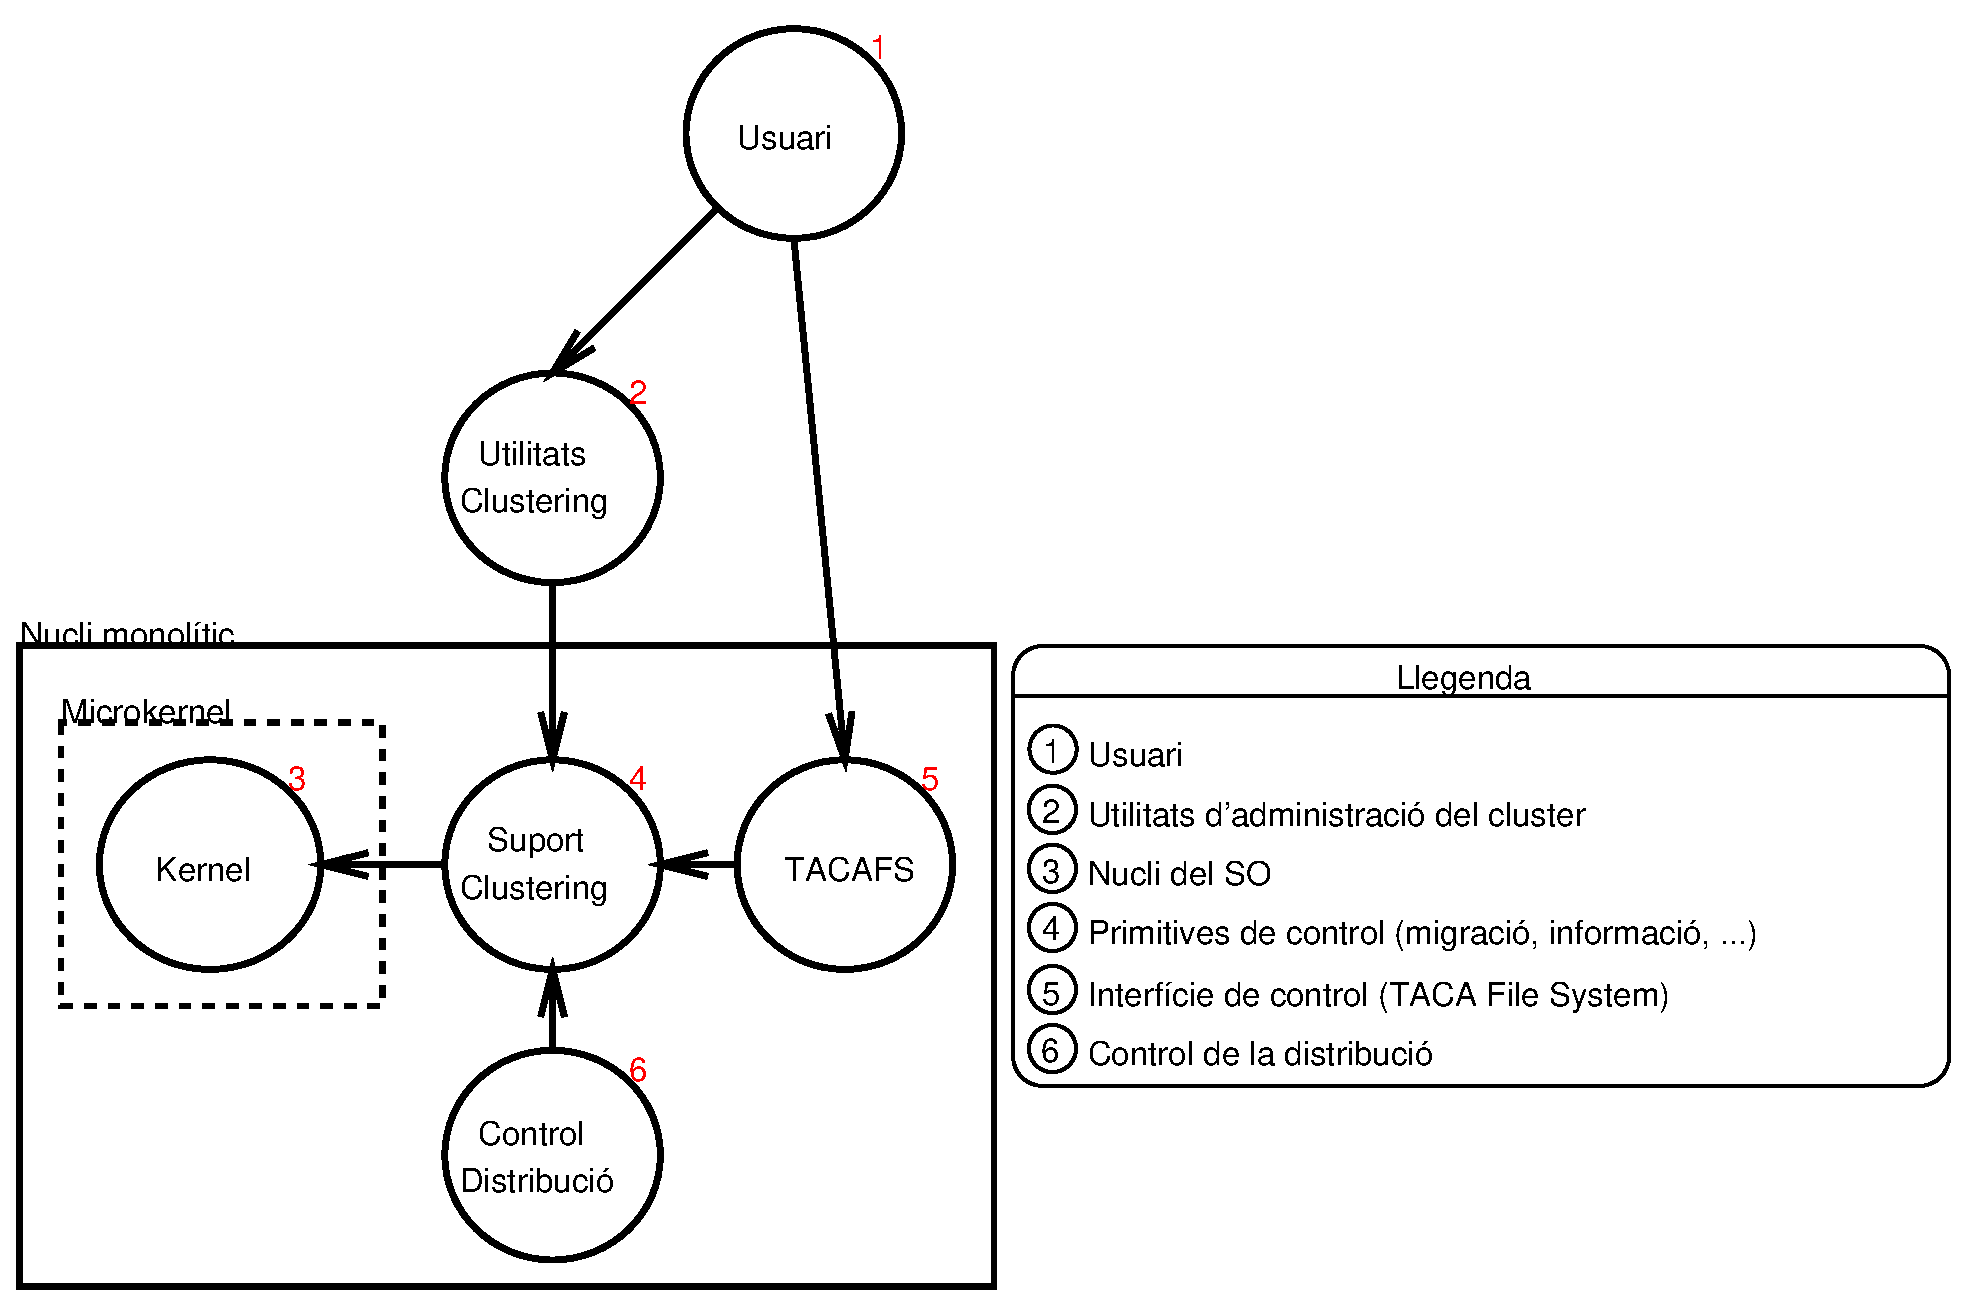
\includegraphics[scale=0.4]{esquema-supcl.eps}
   \caption{Esquema guay}
   \label{fig:esquema-supcl}
\end{figure}

\section{Soluci� super-guay}
En aquest disseny es tracta d'interectuar directament amb el nucli mitjan�ant
elsistema de fitxers virtual /proc.
Seguint amb l'exemple de migraci� de proc�s, en aquest cas es tractaria
d'escriure directament les dades necess�ries al fitxer corresponent del
directori /proc.En aquest cas escrivint el identificador de node al fitxer
"/proc/[PID]/goto" aconseguir�em migrar el proc�s de pid=PID al node desitjat. 

Aquest disseny, respecte l'anterior, aporta simplicitat i independ�ncia respecte
les utilitats que ofereix el cluster i les llibreries. Per� per contra s'hauria
de reescriure molt codi per exemple pel control d'errors, permisos, etc. que ja
estan implementats a les llibreries del software de clustering.

\section{...}

